\documentclass[11pt,a4paper,oneside]{report}

% --- Pacotes de Linguagem e Tipografia ---
\usepackage[utf8]{inputenc}
\usepackage[T1]{fontenc}
\usepackage[brazilian]{babel}

% --- Geometria da Página ---
\usepackage[top=2.5cm, bottom=2.5cm, left=3.0cm, right=2.5cm]{geometry}

% --- Pacotes Matemáticos ---
\usepackage{amsmath, amssymb, amsfonts, amsthm}

% --- Elementos Gráficos e Cores ---
\usepackage{graphicx}
\usepackage{xcolor}
\usepackage{tikz}
\usetikzlibrary{shapes,arrows,positioning,fit,backgrounds,calc}

% --- Definição de Cores Modernas ---
\definecolor{seldonCyan}{HTML}{0891B2}
\definecolor{seldonViolet}{HTML}{7C3AED}
\definecolor{seldonGreen}{HTML}{059669}
\definecolor{seldonAmber}{HTML}{D97706}
\definecolor{seldonDark}{HTML}{0F172A}
\definecolor{codeBg}{HTML}{F8FAFC}
\definecolor{codeFrame}{HTML}{E2E8F0}
\definecolor{boxBg}{HTML}{F0FDF4}

% --- Listagens de Código (listings) ---
\usepackage{listings}
\lstset{
    backgroundcolor=\color{codeBg},
    basicstyle=\ttfamily\footnotesize\color{seldonDark},
    breakatwhitespace=false,
    breaklines=true,
    captionpos=b,
    commentstyle=\color{gray}\itshape,
    keywordstyle=\color{seldonViolet}\bfseries,
    stringstyle=\color{seldonGreen},
    numberstyle=\tiny\color{gray},
    numbers=left,
    numbersep=8pt,
    frame=single,
    rulecolor=\color{codeFrame},
    tabsize=2,
    showstringspaces=false,
    inputencoding=utf8,
    extendedchars=true,
    literate={á}{{\'a}}1 {é}{{\'e}}1 {í}{{\'i}}1 {ó}{{\'o}}1 {ú}{{\'u}}1
             {Á}{{\'A}}1 {É}{{\'E}}1 {Í}{{\'I}}1 {Ó}{{\'O}}1 {Ú}{{\'U}}1
             {ã}{{\~a}}1 {õ}{{\~o}}1 {Ã}{{\~A}}1 {Õ}{{\~O}}1
             {ç}{{\c{c}}}1 {Ç}{{\c{C}}}1 {à}{{\`a}}1 {À}{{\`A}}1
}

% --- Caixas de Destaque Pedagógico (tcolorbox) ---
\usepackage[most]{tcolorbox}
\newtcolorbox{pedagogico}[2][]{
    enhanced,
    colback=seldonCyan!5!white,
    colframe=seldonCyan,
    fonttitle=\bfseries\color{white},
    coltitle=white,
    title=#2,
    arc=4mm,
    boxrule=1pt,
    drop shadow=black!10!white,
    #1
}

\newtcolorbox{casopratico}[2][]{
    enhanced,
    colback=seldonGreen!5!white,
    colframe=seldonGreen,
    fonttitle=\bfseries\color{white},
    coltitle=white,
    title=#2,
    arc=4mm,
    boxrule=1pt,
    drop shadow=black!10!white,
    #1
}

\newtcolorbox{atencao}[1][]{
    enhanced,
    colback=seldonAmber!8!white,
    colframe=seldonAmber,
    fonttitle=\bfseries\color{white},
    coltitle=white,
    title={Atenção \& Boas Práticas de Engenharia},
    arc=3mm,
    boxrule=1pt,
    #1
}

% --- Cabeçalhos e Rodapés ---
\usepackage{fancyhdr}
\setlength{\headheight}{25pt}
\pagestyle{fancy}
\fancyhf{}
\fancyhead[L]{\small\color{gray}\textsl{\leftmark}}
\fancyhead[R]{\small\color{seldonCyan}\textbf{Residência Tecnológica Seldon}}
\fancyfoot[C]{\thepage}
\renewcommand{\headrulewidth}{0.4pt}
\renewcommand{\footrulewidth}{0.4pt}

% --- Formatação de Títulos ---
\usepackage{titlesec}
\titleformat{\chapter}[display]
  {\normalfont\huge\bfseries\color{seldonDark}}
  {\filleft\Huge\color{seldonCyan}\chaptertitlename\ \thechapter}{10pt}
  {\titlerule[1.5pt]\vspace{1.5ex}\filright}
\titleformat{\section}
  {\normalfont\Large\bfseries\color{seldonCyan}}
  {\thesection}{1em}{}
\titleformat{\subsection}
  {\normalfont\large\bfseries\color{seldonViolet}}
  {\thesubsection}{1em}{}

% --- Tabelas e Links ---
\usepackage{booktabs}
\usepackage{tabularx}
\usepackage[colorlinks=true, linkcolor=seldonCyan, citecolor=seldonViolet, urlcolor=seldonGreen]{hyperref}

% --- Informações do Documento ---
\title{
    \textbf{\Huge Residência Tecnológica Seldon}\\[0.5cm]
    \Large\textbf{Manual Técnico Pedagógico Completo}\\
    \large\textit{Android Open Source Project (AOSP), Inteligência Artificial On-Device, Cibersegurança Móvel e Otimização Energética Multiobjetivo}
}
\author{\textbf{Programa de Residência Tecnológica Seldon}}
\date{Outubro de 2026 • 435 Horas de Formação}

\begin{document}

% --- Capa e Folha de Rosto ---
\begin{titlepage}
    \centering
    \vspace*{1.5cm}
    {\Huge\textbf{\color{seldonDark}RESIDÊNCIA TECNOLÓGICA SELDON}\par}
    \vspace{0.8cm}
    {\Large\color{seldonCyan}\textbf{Manual Técnico-Científico \& Pedagógico}\par}
    \vspace{0.3cm}
    {\large Formação Avançada em Android AOSP, Inteligência Artificial, Cibersegurança Móvel e Otimização Energética\par}
    
    \vspace{2cm}
    \begin{tcolorbox}[colback=seldonDark, colframe=seldonCyan, arc=4mm, width=0.9\textwidth]
        \centering\color{white}
        \textbf{\large Estrutura Curricular Integral (435 Horas)}\\[0.3cm]
        \begin{tabular}{ll}
            \textbf{Módulo 1:} Núcleo Comum de Formação & 210h (7 Disciplinas)\\
            \textbf{Módulo 2:} Trilha de Inteligência Artificial & 75h (3 Disciplinas)\\
            \textbf{Módulo 3:} Trilha de Segurança de Dispositivos Móveis & 75h (3 Disciplinas)\\
            \textbf{Módulo 4:} Trilha de Eficiência Energética & 75h (3 Disciplinas)\\
        \end{tabular}
    \end{tcolorbox}

    \vfill
    {\large\textbf{Documento de Referência Curricular e Técnica}\par}
    {\small Baseado no Programa de Pós-Graduação e Formação Tecnológica Seldon\par}
    \vspace{1cm}
    {\large Outubro de 2026\par}
\end{titlepage}

% --- Sumário ---
\tableofcontents
\newpage

% --- Inclusão dos Capítulos ---
\chapter{Módulo 1 – Núcleo Comum de Formação (210 Horas)}
\label{chap:modulo1}

O \textbf{Núcleo Comum de Formação} constitui a base obrigatória e estruturante do programa de Residência Tecnológica Seldon. Seu propósito central é nivelar os residentes em fundamentos sólidos de engenharia de software, rigor do método científico, arquitetura de sistemas móveis, desenvolvimento Android com Kotlin moderno, testes automatizados e gestão ágil de projetos orientada a evidências.

Composto por sete disciplinas complementares que totalizam 210 horas letivas, este módulo estabelece o vocabulário conceitual e a capacitação técnica essenciais para a atuação nas três trilhas de especialização posteriores.

---

\section{Dados, Experimentação e Metodologia Científica (30h)}

\begin{pedagogico}{Objetivo Pedagógico da Disciplina}
Capacitar os residentes para formular problemas de engenharia tecnológica com rigor formal, desenhar ensaios experimentais reprodutíveis, estabelecer métricas objetivas de desempenho e interpretar evidências estatisticamente válidas, respeitando os preceitos de propriedade intelectual.
\end{pedagogico}

\subsection{Formulação de Problemas Tecnológicos e Hipóteses}
Na engenharia de software contemporânea, decisões arquiteturais e otimizações de baixo nível não podem se basear em intuição empírica desprovida de validação formal. O método científico aplicado a sistemas computacionais exige a estruturação de hipóteses estatísticas verificáveis:
\begin{itemize}
    \item \textbf{Hipótese Nula ($H_0$):} Postula que a modificação introduzida (ex.: nova estratégia de compactação de memória ou novo algoritmo de renderização) não produz diferença estatisticamente significativa no parâmetro de interesse em comparação com a linha de base (\textit{baseline}).
    \item \textbf{Hipótese Alternativa ($H_1$):} Postula que a intervenção tecnológica produz um efeito real mensurável (redução de latência, menor variabilidade temporal ou conservação de energia).
\end{itemize}

\subsection{Desenho Experimental e Variáveis de Controle}
O isolamento de ruído em plataformas móveis como o Android é um dos desafios mais complexos na coleta de métricas, devido a variáveis intervenientes não controladas:
\begin{enumerate}
    \item \textbf{Variável Independente ($X$):} O fator sob manipulação direta do pesquisador (ex.: uso de \texttt{LazyColumn} em Jetpack Compose versus \texttt{RecyclerView} tradicional).
    \item \textbf{Variável Dependente ($Y$):} A métrica de resposta observada (ex.: tempo de renderização por quadro $T_{\text{frame}}$ em milissegundos).
    \item \textbf{Variáveis de Controle e Ruído:} Fatores externos que devem ser congelados durante o ensaio:
    \begin{itemize}
        \item Nível e temperatura da bateria (para evitar \textit{thermal throttling});
        \item Frequência de clock da CPU fixada via \texttt{cpufreq} no kernel;
        \item Brilho da tela fixado e rádio celular configurado em modo avião.
    \end{itemize}
\end{enumerate}

\begin{figure}[htbp]
\centering
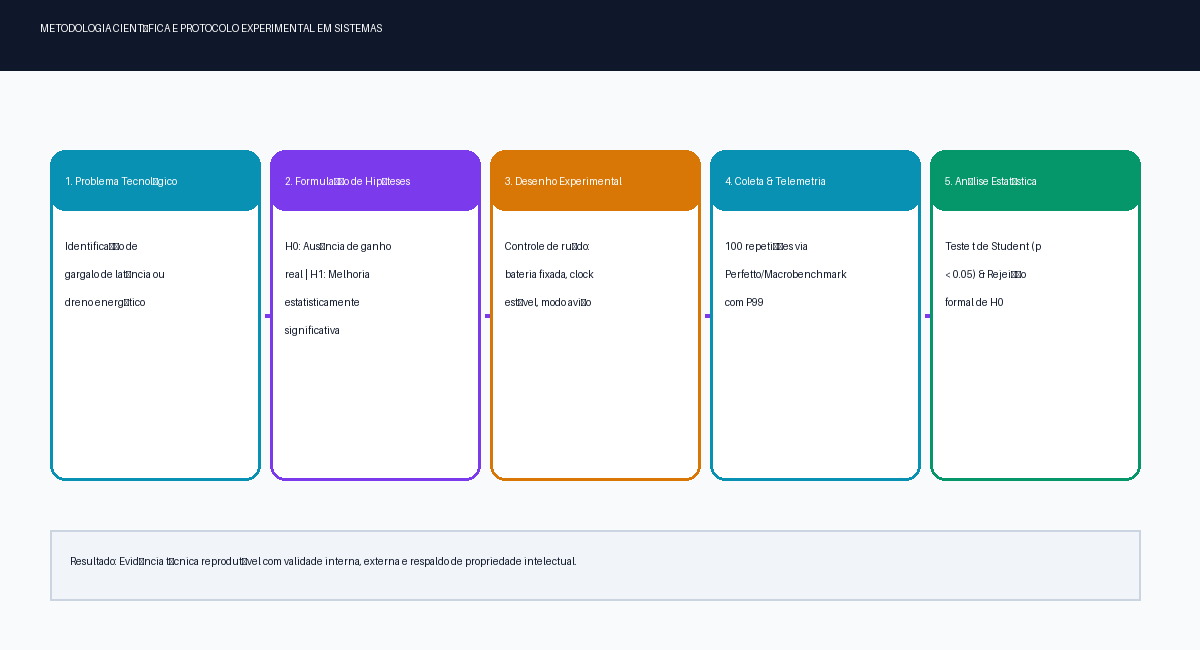
\includegraphics[width=0.95\textwidth]{imagens/fig_metodologia_cientifica.png}
\caption{Fluxograma do Protocolo Experimental Rigoroso: formulação de hipóteses estatísticas, controle de ruído térmico/clock e validação via Teste $t$ de Student ($p < 0{,}05$).}
\label{fig:metodologia}
\end{figure}

\subsection{Análise Estatística Inferencial: Teste $t$ de Student e ANOVA}
Para rejeitar formalmente a hipótese nula $H_0$ com nível de significância $\alpha = 0{,}05$, calcula-se a estatística $t$ para duas amostras independentes com variâncias populacionais desconhecidas:
\begin{equation}
    t = \frac{\bar{X}_1 - \bar{X}_2}{\sqrt{\frac{s_1^2}{n_1} + \frac{s_2^2}{n_2}}}
\end{equation}
onde $\bar{X}_i$ representa a média amostral, $s_i^2$ a variância amostral e $n_i$ o tamanho de cada lote de medição. A rejeição de $H_0$ ocorre quando o $p$-valor associado à distribuição $t$ com os respectivos graus de liberdade for estritamente menor que $\alpha$, comprovando que o ganho de desempenho não decorreu de mero acaso estocástico.

\begin{casopratico}{Caso Prático: Protocolo Experimental de Frame Jank}
\textbf{Cenário:} Comprovar se uma alteração na alocação de objetos em um loop gráfico reduz a taxa de quadros engasgados (\textit{jank frames}).\\
\textbf{Protocolo:} 100 repetições de um teste automatizado via \texttt{macrobenchmark}. Registro dos tempos no percentil 99 ($P_{99}$).\\
\textbf{Resultado:} $\bar{X}_{\text{antigo}} = 24{,}8\text{ ms}$, $\bar{X}_{\text{novo}} = 14{,}2\text{ ms}$. Estatística $t = 12{,}4$, resultando em $p < 0{,}001$. Conclusão: a hipótese nula é categoricamente rejeitada com 99{,}9\% de confiança estatística.
\end{casopratico}

---

\section{Engenharia de Software, Requisitos e Gestão do Desenvolvimento (24h)}

\begin{pedagogico}{Objetivo Pedagógico da Disciplina}
Desenvolver competências para elicitar, analisar e formalizar requisitos de software complexos, estruturar ciclos de desenvolvimento ágeis sustentáveis e assegurar a rastreabilidade bidirecional contínua entre o desafio industrial e a entrega executável.
\end{pedagogico}

\subsection{Engenharia de Requisitos Funcionais e Não Funcionais}
Em sistemas de missão crítica e plataformas embarcadas, a especificação precisa de requisitos constitui o primeiro baluarte contra falhas catastróficas:
\begin{itemize}
    \item \textbf{Requisitos Funcionais (RF):} Descrevem os comportamentos intrínsecos do software (ex.: ``O sistema deve sincronizar os dados biométricos com a nuvem a cada 15 minutos se houver conexão Wi-Fi'').
    \item \textbf{Requisitos Não Funcionais (RNF):} Estabelecem restrições de qualidade, tais como:
    \begin{itemize}
        \item Latência de resposta da interface gráfica $\le 16{,}6\text{ ms}$ em 60 Hz;
        \item Consumo de corrente em repouso com tela apagada $\le 15\text{ mA}$;
        \item Ocupação máxima em memória residente (RSS) $\le 64\text{ MB}$.
    \end{itemize}
\end{itemize}

\subsection{Matriz de Rastreabilidade de Requisitos (RTM)}
A rastreabilidade bidirecional é implementada através de identificadores unívocos que conectam cada necessidade do projeto ao seu artefato de verificação:
\begin{equation}
    \text{Desafio Industrial} \longrightarrow \text{RF/RNF} \longrightarrow \text{User Story} \longrightarrow \text{Branch/Commit} \longrightarrow \text{Teste Automatizado}
\end{equation}

\begin{lstlisting}[language=bash, caption={Estrutura de Rastreabilidade em Commits Git}]
# Formato de mensagem de commit em conformidade com RTM:
feat(power): [RF-042][REQ-BAT-09] migra polling para WorkManager com restricao de carga

- Substitui ScheduledExecutorService por PeriodicWorkRequestBuilder
- Garante execucao exclusivamente quando o device estiver carregando e em Wi-Fi
- Evita dreno em background (RNF-ENG-03)
- Testes unitarios automatizados em WorkManagerTest.kt (Cobertura 100%)
\end{lstlisting}

---

\section{Metodologia de Projetos, Ética e Habilidades Profissionais (30h)}

\begin{pedagogico}{Objetivo Pedagógico da Disciplina}
Preparar o residente para liderar e colaborar em equipes multidisciplinares sob a metodologia de Aprendizagem Baseada em Projetos (PBL), mantendo rigor ético profissional, governança de dados conforme a LGPD e documentação formal de decisões arquiteturais.
\end{pedagogico}

\subsection{Aprendizagem Baseada em Projetos (PBL) na Residência}
Diferente da pedagogia passiva tradicional, o PBL imerge os residentes em problemas reais trazidos por parceiros industriais. O ciclo de aprendizado estrutura-se em:
\begin{enumerate}
    \item \textbf{Imersão e Delimitação:} Análise do problema e formulação de perguntas norteadoras.
    \item \textbf{Planejamento e Decomposição:} Criação de \textit{Product Backlog} e definição de papéis (Product Owner, Tech Lead, Especialista em QA).
    \item \textbf{Ciclos de Prototipação e Experimentação:} \textit{Sprints} quinzenais com geração de evidências técnicas tangíveis.
    \item \textbf{Apresentação de Resultados \& Retrospectiva:} Demonstrações técnicas para bancas de avaliação acadêmica e corporativa.
\end{enumerate}

\subsection{Governança de Dados e Conformidade com a LGPD}
O desenvolvimento para dispositivos móveis envolve acesso a sensores sensíveis (GPS, câmera, microfone, identificadores de rádio). A Lei Geral de Proteção de Dados Pessoais (Lei nº 13.709/2018) impõe diretrizes estritas:
\begin{itemize}
    \item \textbf{Privacy by Design:} Anonimização na borda através de funções de dispersão criptográfica (SHA-256 com \textit{salt} local);
    \item \textbf{Minimização da Coleta:} Coleta estritamente restrita aos dados indispensáveis à execução do serviço contratado;
    \item \textbf{Relatório de Impacto à Proteção de Dados (RIPD):} Documentação formal descrevendo os fluxos de tratamento de dados e as salvaguardas tecnológicas implementadas.
\end{itemize}

---

\section{Arquitetura de Software (18h)}

\begin{pedagogico}{Objetivo Pedagógico da Disciplina}
Capacitar os residentes na aplicação de princípios SOLID, arquiteturas desacopladas (Clean Architecture, MVVM e MVI) e injeção de dependências em aplicações Android escaláveis e de alta testabilidade.
\end{pedagogico}

\subsection{Clean Architecture no Ecossistema Android}
A Clean Architecture preconiza a separação concêntrica de responsabilidades, assegurando que o núcleo de regras de negócio (\textit{Domain}) permaneça agnóstico a detalhes de infraestrutura (bancos de dados, redes e frameworks de UI):

\begin{figure}[htbp]
\centering
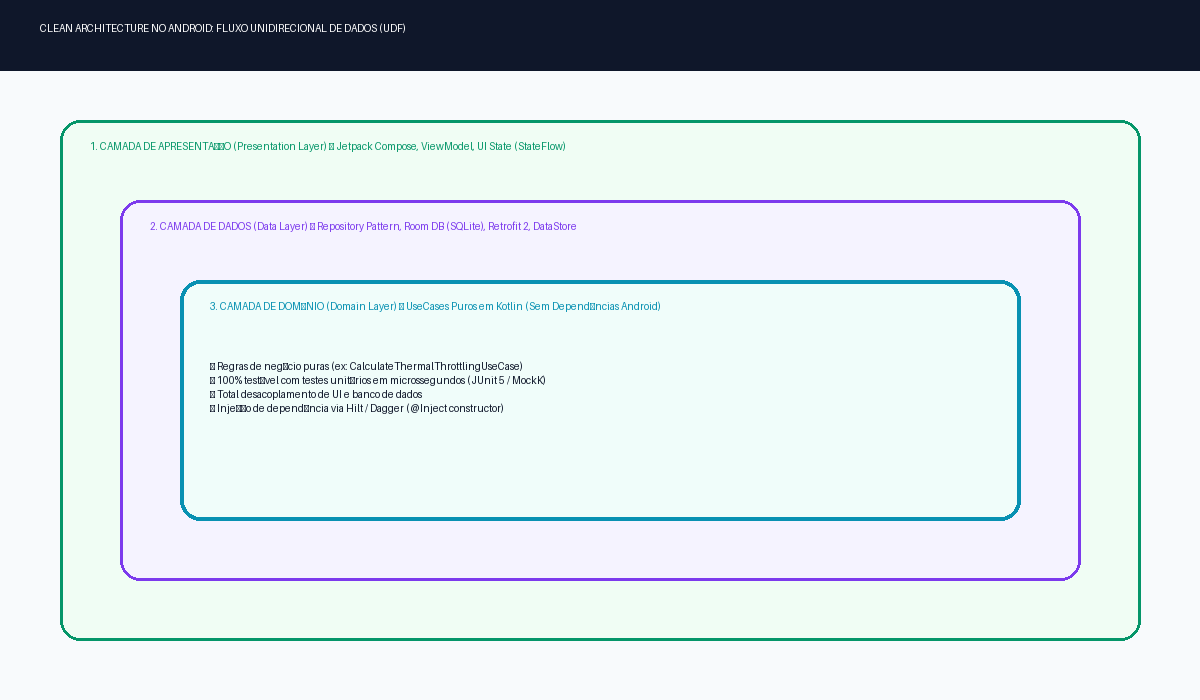
\includegraphics[width=0.95\textwidth]{imagens/fig_clean_architecture.png}
\caption{Diagrama de Camadas da Clean Architecture no Android: a camada de Domínio pura encapsulada pelas camadas de Dados e Apresentação com fluxo unidirecional.}
\label{fig:clean_arch}
\end{figure}

\subsection{Implementação Prática: UseCase Puro com Kotlin}
\begin{lstlisting}[language=Java, caption={Implementação de UseCase na Camada de Domínio}]
package com.seldon.domain.usecase

import com.seldon.domain.model.ThermalThrottlingEvent
import com.seldon.domain.repository.SensorTelemetryRepository
import javax.inject.Inject

/**
 * Regra de negócio pura: avalia risco termico sem acoplamento ao Android SDK.
 */
class EvaluateThermalRiskUseCase @Inject constructor(
    private val telemetryRepository: SensorTelemetryRepository
) {
    suspend operator fun invoke(thresholdCelsius: Double): ThermalThrottlingEvent {
        val currentTemperature = telemetryRepository.readSocTemperature()
        val isCritical = currentTemperature >= thresholdCelsius
        
        return ThermalThrottlingEvent(
            currentTemperature = currentTemperature,
            threshold = thresholdCelsius,
            requiresIntervention = isCritical
        )
    }
}
\end{lstlisting}

---

\section{Inteligência Artificial: Fundamentos, Frameworks e Aplicações (36h)}

\begin{pedagogico}{Objetivo Pedagógico da Disciplina}
Compreender a esteira completa de engenharia de Machine Learning e Deep Learning, desde a preparação de tensores de dados até o treinamento, validação cruzada, regularização e consumo de inferências preditivas integradas a aplicações móveis.
\end{pedagogico}

\subsection{O Pipeline Clássico de Aprendizado Supervisionado}
O aprendizado de máquina supervisionado visa estimar uma função $f: \mathcal{X} \to \mathcal{Y}$ que mapeie um vetor de características $\mathbf{x} \in \mathbb{R}^d$ em um rótulo $y \in \mathcal{Y}$. Em problemas de classificação, minimiza-se a função de perda de entropia cruzada (\textit{Cross-Entropy Loss}):
\begin{equation}
    \mathcal{L}_{\text{CE}}(\mathbf{w}) = -\frac{1}{N} \sum_{i=1}^{N} \sum_{k=1}^{K} y_{i,k} \log\left(\hat{y}_{i,k}(\mathbf{w})\right)
\end{equation}
onde $N$ é o número de amostras, $K$ o número de classes e $\hat{y}_{i,k}$ a probabilidade predita pelo modelo parametrizado pelos pesos $\mathbf{w}$.

\subsection{Matriz de Confusão e Métricas de Validação Rigorosas}
Em sistemas operacionais, a ocorrência de anomalias (quedas bruscas de tensão ou travamentos) representa eventos raros (dados altamente desbalanceados). A acurácia global é inadequada; priorizam-se:
\begin{equation}
    \text{Precision} = \frac{\text{VP}}{\text{VP} + \text{FP}}, \quad \text{Recall} = \frac{\text{VP}}{\text{VP} + \text{FN}}, \quad F_1\text{-Score} = 2 \cdot \frac{\text{Precision} \cdot \text{Recall}}{\text{Precision} + \text{Recall}}
\end{equation}

---

\section{Programação Java/Kotlin e Desenvolvimento de Aplicações Android (42h)}

\begin{pedagogico}{Objetivo Pedagógico da Disciplina}
Capacitar os residentes na construção de aplicações Android modernas com Kotlin, arquitetura baseada em Coroutines e Flow, interface declarativa com Jetpack Compose e domínio profundo dos quatro componentes canônicos do AOSP.
\end{pedagogico}

\subsection{Os Quatro Componentes Canônicos do AOSP}
\begin{figure}[htbp]
\centering
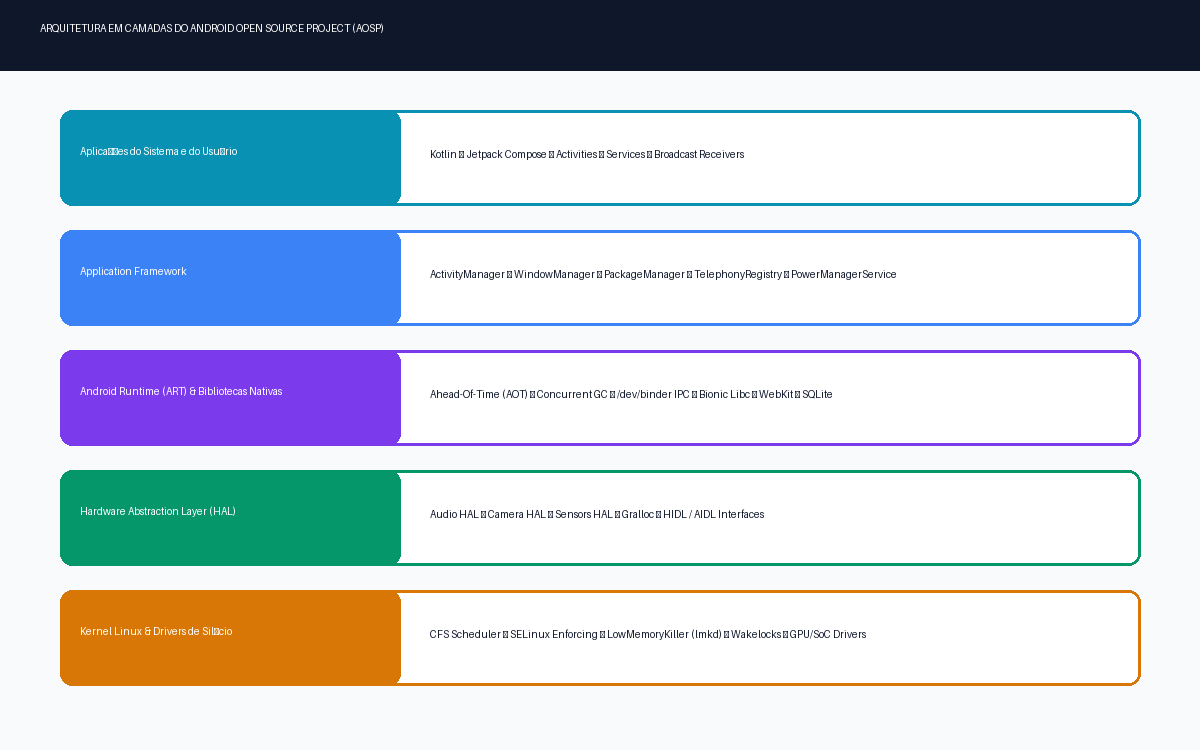
\includegraphics[width=0.95\textwidth]{imagens/fig_aosp_arquitetura.png}
\caption{Visão Geral da Pilha Arquitetural do AOSP: desde o Kernel Linux e HAL até o Android Runtime (ART) e o Application Framework.}
\label{fig:aosp_stack_cap1}
\end{figure}

O ecossistema Android fundamenta-se em quatro pilares declarados no \texttt{AndroidManifest.xml}:
\begin{enumerate}
    \item \textbf{Activity:} Representa uma interface gráfica com o usuário e controla o fluxo de vida visual (\texttt{onCreate}, \texttt{onStart}, \texttt{onResume}, etc.);
    \item \textbf{Service:} Executa processamento contínuo em segundo plano sem interface gráfica (ex.: serviços de telemetria ou reprodução de áudio);
    \item \textbf{Broadcast Receiver:} Permite à aplicação receber anúncios de eventos do sistema ou de outros apps (ex.: \texttt{ACTION\_BATTERY\_LOW}, \texttt{CONNECTIVITY\_CHANGE});
    \item \textbf{Content Provider:} Gerencia o acesso seguro e estruturado a repositórios de dados compartilhados entre processos distintos.
\end{enumerate}

\subsection{Interface Reativa com Jetpack Compose e StateFlow}
O Jetpack Compose adota o paradigma declarativo: a interface visual é uma função pura do estado atual $UI = f(State)$.

\begin{lstlisting}[language=Java, caption={Exemplo de ViewModel reativa com StateFlow em Kotlin}]
class TelemetryViewModel @Inject constructor(
    private val evaluateThermalRiskUseCase: EvaluateThermalRiskUseCase
) : ViewModel() {

    private val _uiState = MutableStateFlow<TelemetryUiState>(TelemetryUiState.Loading)
    val uiState: StateFlow<TelemetryUiState> = _uiState.asStateFlow()

    fun triggerAnalysis() {
        viewModelScope.launch {
            try {
                val result = evaluateThermalRiskUseCase(thresholdCelsius = 42.0)
                _uiState.value = TelemetryUiState.Success(result)
            } catch (e: Exception) {
                _uiState.value = TelemetryUiState.Error(e.localizedMessage)
            }
        }
    }
}
\end{lstlisting}

---

\section{Testes, Automação, Segurança e Integração Contínua (30h)}

\begin{pedagogico}{Objetivo Pedagógico da Disciplina}
Compreender e implementar esteiras de automação de testes unitários, instrumentados e de integração contínua (CI/CD), aplicando análise estática de código e boas práticas de segurança defensiva.
\end{pedagogico}

\subsection{A Pirâmide de Testes no Android}
Uma estratégia eficiente de garantia de qualidade balanceia velocidade de execução com fidelidade de ambiente:
\begin{itemize}
    \item \textbf{Testes Unitários (Base - 70\%):} Executam na JVM local em milissegundos utilizando JUnit 5 e MockK. Validam regras de negócio puras;
    \item \textbf{Testes de Integração / Robolectric (Meio - 20\%):} Simulam classes do SDK Android na JVM sem necessitar de emulador ou dispositivo físico;
    \item \textbf{Testes E2E Instrumentados (Topo - 10\%):} Executam diretamente no dispositivo via Espresso ou UIAutomator, validando fluxos críticos de ponta a ponta.
\end{itemize}

\subsection{Pipeline CI/CD Automatizado com GitHub Actions}
\begin{lstlisting}[language=bash, caption={Etapas Críticas de uma Pipeline CI/CD Android}]
# Workflow de validacao continua no GitHub Actions:
name: Android CI Pipeline
on: [push, pull_request]

jobs:
  validate:
    runs-on: ubuntu-latest
    steps:
      - uses: actions/checkout@v4
      - uses: actions/setup-java@v4
        with: { java-version: '17', distribution: 'temurin' }
      - name: Analise Estatica (Detekt & Lint)
        run: ./gradlew detekt lintRelease
      - name: Testes Unitarios
        run: ./gradlew testReleaseUnitTest
      - name: Build do APK de Release
        run: ./gradlew assembleRelease
\end{lstlisting}

\chapter{Módulo 2 – Trilha de IA aplicada à Otimização de Sistemas Android (75 Horas)}
\label{chap:modulo2}

A \textbf{Trilha de Inteligência Artificial aplicada à Otimização de Sistemas Android} explora o coração do sistema operacional, focando no \textbf{Android Open Source Project (AOSP)}. Os residentes aprendem a extrair telemetria em nanossegundos do kernel Linux e do runtime ART, modelar padrões complexos de uso com redes neurais profundas e converter esses modelos em artefatos quantizados ultracompactos capazes de rodar em tempo real na NPU do dispositivo móvel com baixíssimo impacto energético.

---

\section{AOSP – Observabilidade e Desempenho (25h)}

\begin{pedagogico}{Objetivo Pedagógico da Disciplina}
Compreender a arquitetura interna do Android em profundidade, dominar o mecanismo de comunicação interprocessos (Binder IPC), analisar o ciclo de vida da memória física via Low Memory Killer (LMK) e diagnosticar gargalos de desempenho e quedas de quadros com a ferramenta de rastreamento Perfetto.
\end{pedagogico}

\subsection{A Arquitetura em Camadas do AOSP}
O Android não é uma distribuição Linux convencional; ele implementa uma pilha de abstrações concebida para segurança, desacoplamento de hardware e isolamento de processos:
\begin{enumerate}
    \item \textbf{Kernel Linux:} Gerencia agendamento de processos (CFS), drivers de silício, gerenciamento de energia e contém o driver `/dev/binder`;
    \item \textbf{Hardware Abstraction Layer (HAL):} Módulos C/C++ que expõem APIs genéricas para a plataforma (câmera, áudio, sensores) ocultando especificidades proprietárias dos semicondutores;
    \item \textbf{Android Runtime (ART) \& Bionic Libc:} Motor de execução que compila bytecode DEX para código nativo (AOT/JIT) e provê Garbage Collection concorrente sem pausas longas;
    \item \textbf{Application Framework:} Serviços de sistema nativos executados pelo processo central \texttt{system\_server} (ActivityManagerService, WindowManagerService, PowerManagerService);
    \item \textbf{Aplicações:} Processos em espaço de usuário, cada qual encapsulado em sua própria jaula de permissões (UID Unix único).
\end{enumerate}

\subsection{O Mecanismo de Comunicação Inter-Processos: Binder IPC}
Como cada aplicativo e serviço de sistema roda em seu próprio processo isolado, qualquer interação entre eles exige IPC (\textit{Inter-Process Communication}). O mecanismo padrão do Unix (sockets, pipes) impõe duas cópias de memória no kernel (espaço de usuário A $\to$ kernel $\to$ espaço de usuário B), gerando degradação inaceitável.

O AOSP resolve este problema através do **Binder IPC**, que utiliza **compartilhamento de memória com cópia única (\textit{single-copy}) ou Zero-Copy**:

\begin{figure}[htbp]
\centering
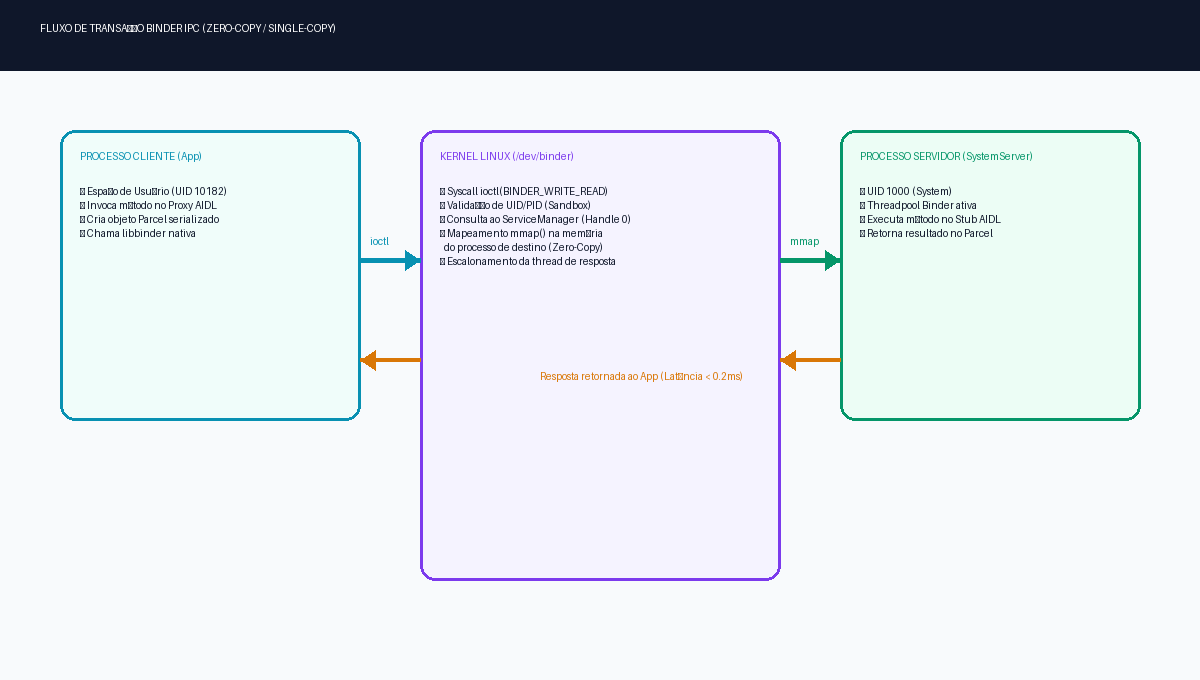
\includegraphics[width=0.95\textwidth]{imagens/fig_binder_ipc.png}
\caption{Fluxo Detalhado de Transação IPC no AOSP via driver \texttt{/dev/binder}: empacotamento em Parcel, syscall \texttt{ioctl}, resolução no ServiceManager e entrega Zero-Copy via \texttt{mmap} compartilhado.}
\label{fig:binder_flow_img}
\end{figure}

O cliente prepara uma estrutura de dados serializada chamada \texttt{Parcel}. Através da interface AIDL (\textit{Android Interface Definition Language}), o código Kotlin invoca um método local no \textit{Proxy}, que empacota os argumentos e realiza a chamada de sistema \texttt{ioctl(fd, BINDER\_WRITE\_READ, \&bwr)}. O kernel localiza a página de memória do processo destino pré-alocada via \texttt{mmap()} e grava os dados diretamente nela, acordando uma thread da threadpool do servidor para executar o \textit{Stub}.

\subsection{Observabilidade em Nanossegundos com Perfetto Trace}
\begin{figure}[htbp]
\centering
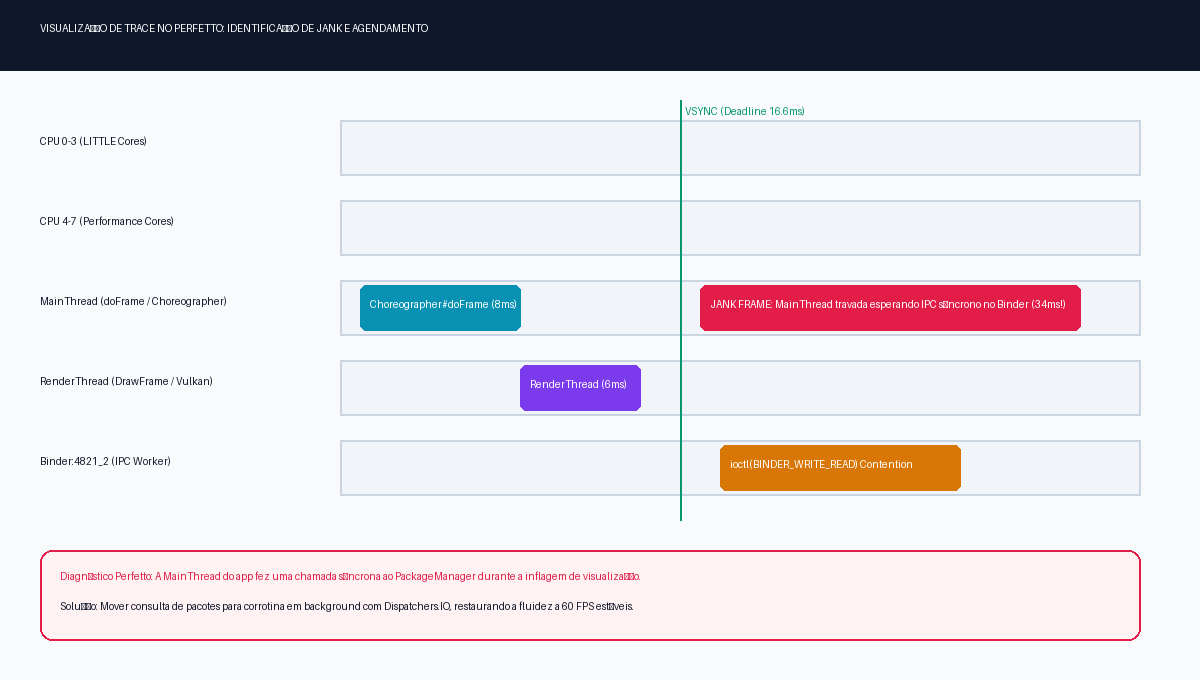
\includegraphics[width=0.95\textwidth]{imagens/fig_perfetto_timeline.png}
\caption{Rastreamento de Execução no Perfetto: identificação visual de contenção de lock no barramento Binder e diagnóstico de queda de quadros (\textit{jank frame}) violando o deadline de 16.6ms.}
\label{fig:perfetto_trace_img}
\end{figure}
Para diagnosticar gargalos que degradam a taxa de 60 ou 120 quadros por segundo (onde cada quadro dispõe de apenas $16{,}6\text{ ms}$ ou $8{,}3\text{ ms}$), utiliza-se o **Perfetto**:
\begin{itemize}
    \item Gravação de rastros baseada no subsistema \texttt{ftrace} do kernel;
    \item Eventos de agendamento de CPU: \texttt{sched\_switch} e \texttt{sched\_wakeup};
    \item Transações de Binder: visualização do tempo de espera e fila de atendimento;
    \item \textit{Choreographer} e \textit{RenderThread}: rastreamento de \texttt{doFrame}, inflamento de views e chamadas de desenho OpenGL/Vulkan.
\end{itemize}

---

\section{Aprendizado de Máquina e Aprendizado Profundo (30h)}

\begin{pedagogico}{Objetivo Pedagógico da Disciplina}
Capacitar os residentes a projetar, treinar e validar redes neurais profundas aplicadas à detecção de anomalias operacionais e predição de comportamento em sistemas Android, tratando dados ruidosos de telemetria.
\end{pedagogico}

\subsection{Detecção de Anomalias com Autoencoders Neurais}
Uma das aplicações de IA no AOSP é detectar quando um aplicativo entra em um estado anômalo de dreno silencioso de bateria ou vazamento de recursos. Para tal, treina-se um **Autoencoder** exclusivamente com dados de operação nominal:

\begin{equation}
    \mathbf{z} = \sigma(\mathbf{W}_e \mathbf{x} + \mathbf{b}_e) \quad \text{(Codificador)}
\end{equation}
\begin{equation}
    \hat{\mathbf{x}} = \sigma(\mathbf{W}_d \mathbf{z} + \mathbf{b}_d) \quad \text{(Decodificador)}
\end{equation}
onde $\mathbf{x} \in \mathbb{R}^d$ é o vetor de métricas instantâneas (uso de CPU por core, taxa de interrupts, frequência de chamadas IPC Binder). O modelo é treinado para minimizar o Erro Quadrático Médio de reconstrução (\textit{Reconstruction Error}):
\begin{equation}
    \text{MSE}(\mathbf{x}, \hat{\mathbf{x}}) = \frac{1}{d} \sum_{j=1}^{d} (x_j - \hat{x}_j)^2
\end{equation}

---

\section{IA On-device e Otimização de Modelos (20h)}

\begin{pedagogico}{Objetivo Pedagógico da Disciplina}
Dominar as técnicas de engenharia para adaptação de modelos neurais em dispositivos móveis, aplicando quantização afim de inteiros (INT8), poda esparsa de conexões sinápticas e delegação de tensores para a NPU via Android NNAPI e LiteRT.
\end{pedagogico}

\subsection{Teoria Matemática da Quantização Afim \texorpdfstring{(FP32 $\to$ INT8)}{(FP32 para INT8)}}
\begin{figure}[htbp]
\centering
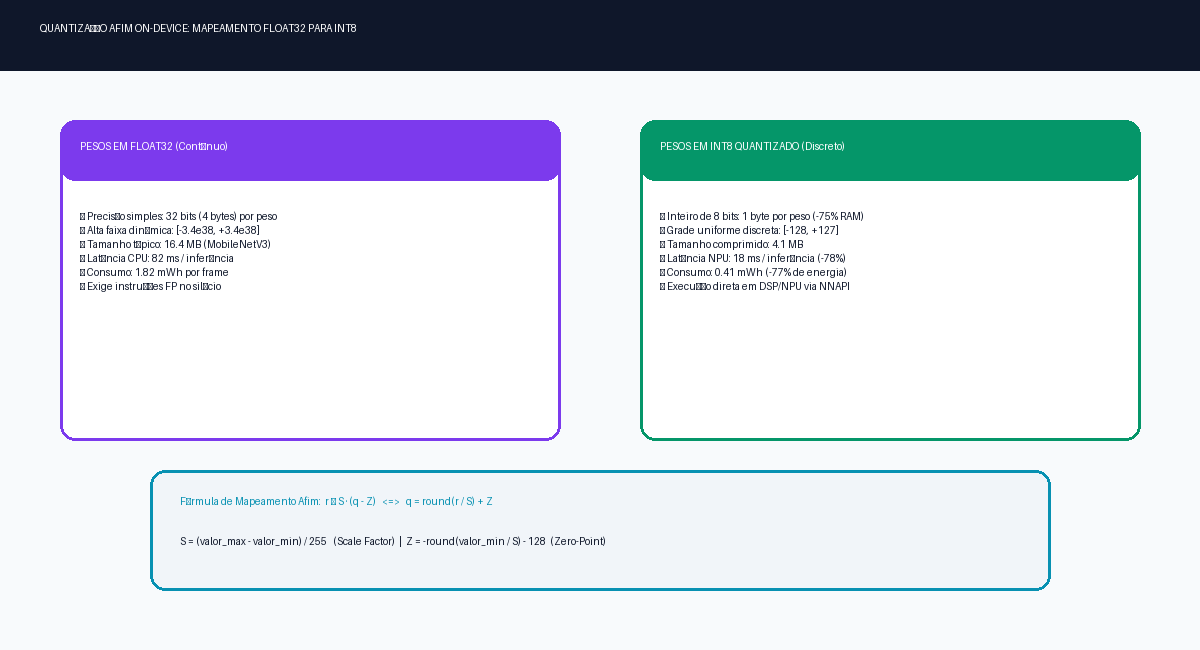
\includegraphics[width=0.95\textwidth]{imagens/fig_quantizacao_neural.png}
\caption{Mapeamento Afim de Quantização On-Device: conversão de tensores contínuos em Float32 para inteiros uniformes em INT8, exibindo redução de 75\% no tamanho e aceleração via NNAPI.}
\label{fig:quantizacao_img}
\end{figure}

Modelos neurais convencionais operam com tensores em ponto flutuante de precisão simples (\texttt{Float32}, ocupando 4 bytes por parâmetro). Em smartphones, essa representação consome banda excessiva de memória RAM e dissipa calor desnecessário.

A **Quantização Afim de Inteiros (Uniform Affine Quantization)** mapeia um valor real contínuo $r \in [\alpha, \beta]$ em um inteiro de 8 bits $q \in [-128, 127]$ através da relação linear:
\begin{equation}
    r \approx S \cdot (q - Z)
\end{equation}
onde $S = \frac{\beta - \alpha}{255}$ é o fator de escala e $Z = \text{round}\left( -\frac{\alpha}{S} \right) + q_{\text{min}}$ é o ponto zero.

---

\section{Revisão da Literatura e Estado da Arte: IA e Observabilidade em SO}

A literatura científica recente converge para a necessidade de observabilidade profunda com overhead desprezível e inferência inteligente descentralizada:
\begin{itemize}
    \item \textbf{Observabilidade em Kernel e Sistemas Operacionais:} \cite{gregg2019bpf} demonstra que ferramentas tradicionais baseadas em amostragem periódica de \texttt{/proc} introduzem distorções severas de amostragem (\textit{observer effect}). O uso de pontos de rastreamento estáticos (\textit{tracepoints}) e buffers circulares sem bloqueio no kernel Linux — como implementado no Perfetto — viabiliza capturar eventos em nanossegundos com consumo de CPU inferior a $1{,}5\%$.
    \item \textbf{Detecção Não-Supervisionada de Anomalias em Telemetria:} \cite{malhotra2016lstm} e \cite{zhou2017anomaly} comprovaram que redes neurais autoassociativas (Autoencoders e LSTM Encoder-Decoders) superam métodos estatísticos clássicos (como limites baseados em desvio padrão $\mu \pm 3\sigma$) na detecção de falhas silenciosas em séries temporais multidimensionais, pois aprendem correlações intrínsecas e não-lineares entre subsistemas heterogêneos.
    \item \textbf{Quantização com Aritmética de Inteiros Acelerada:} O trabalho seminal de \cite{jacob2018quantization} estabeleceu as bases formais da quantização afim adotada pelo Google no ecossistema Android/LiteRT, comprovando que a substituição de instruções de ponto flutuante por aritmética de inteiros INT8 com multiplicadores de ponto fixo reduz em $75\%$ o consumo de largura de banda de memória e acelera em mais de $4\times$ a execução em aceleradores de hardware como NPUs e DSPs, preservando mais de $99\%$ da acurácia original de redes complexas como MobileNet.
\end{itemize}

---

\section{Arquitetura de Engenharia do Projeto Final: Seldon Anomaly Watcher}

Como projeto final de conclusão do Módulo 2, os residentes projetam e implementam o **Seldon Anomaly Watcher**, uma solução completa de governança inteligente embarcada no AOSP.

\begin{figure}[htbp]
\centering
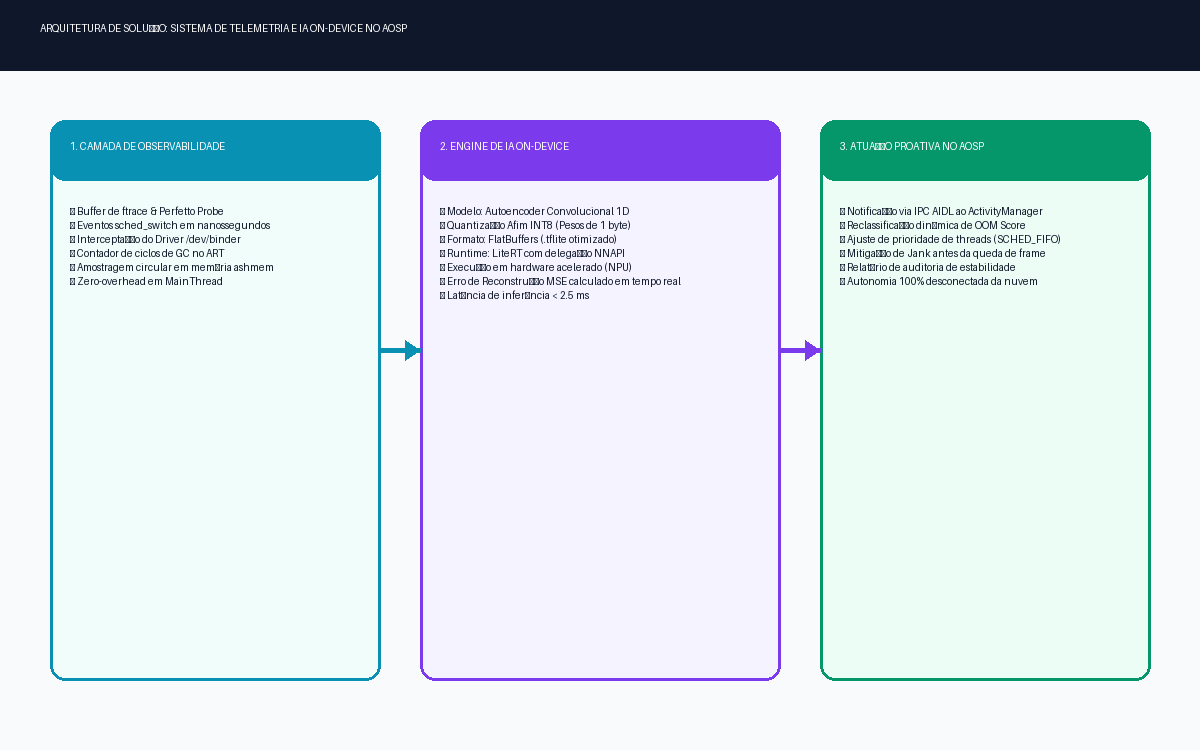
\includegraphics[width=0.95\textwidth]{imagens/fig_arq_projeto_ia.png}
\caption{Arquitetura de Engenharia do Projeto Final (Módulo 2): Pipeline completo desde a captura de telemetria no kernel via Perfetto até a inferência quantizada em NPU e atuação corretiva no System Server.}
\label{fig:arq_ia_projeto}
\end{figure}

\subsection{Especificação Técnica dos Módulos da Solução}
A arquitetura estrutura-se em três subsistemas desacoplados:
\begin{enumerate}
    \item \textbf{Coletor de Telemetria de Baixo Nível (Kernel Probe):}
    \begin{itemize}
        \item Consome dados de \texttt{tracefs} e eventos \texttt{sched\_switch}, calculando a duração das fatias de tempo (\textit{timeslices}) de cada thread em execução;
        \item Monitora transações no driver \texttt{/dev/binder}, registrando tempos de espera síncronos e tamanho dos buffers transmitidos;
        \item Grava vetores de atributos em janelas deslizantes de $500\text{ ms}$ em memória compartilhada (\textit{ashmem}).
    \end{itemize}
    \item \textbf{Engine de Inferência On-Device (LiteRT + NNAPI):}
    \begin{itemize}
        \item Executa o modelo Autoencoder Convolucional 1D quantizado em INT8 (\texttt{anomaly\_detector\_v2.tflite});
        \item Delegado via driver Android NNAPI diretamente para a NPU do chipset;
        \item Computa o erro de reconstrução instantâneo $\text{MSE}_t$; se $\text{MSE}_t > \tau_{\text{critico}}$, dispara um evento de anomalia estruturado.
    \end{itemize}
    \item \textbf{Atuador Proativo de Políticas AOSP (System Server Handler):}
    \begin{itemize}
        \item Recebe o alerta via interface AIDL \texttt{ISeldonPolicyCallback};
        \item Reclassifica preventivamente a prioridade de agendamento de threads com risco de jank de \texttt{SCHED\_OTHER} para \texttt{SCHED\_FIFO};
        \item Notifica o \texttt{ActivityManagerService} para contenção de tarefas em segundo plano causadoras de concorrência excessiva de locks.
    \end{itemize}
\end{enumerate}

\chapter{Módulo 3 – Trilha de Segurança de Dispositivos Móveis e Automação (75 Horas)}
\label{chap:modulo3}

A \textbf{Trilha de Segurança de Dispositivos Móveis e Automação de Validações} aborda a defesa em profundidade da plataforma Android. Os residentes aprendem a modelar vetores de ataque, auditar superfícies expostas, desvendar os mecanismos de proteção do kernel Linux (SELinux e Sandbox), explorar o isolamento criptográfico por hardware (\textit{StrongBox} e \textit{Keystore}) e automatizar verificações contínuas em pipelines DevSecOps.

---

\section{Introdução à Cibersegurança, Modelagem de Ameaças e Vulnerabilidades (35h)}

\begin{pedagogico}{Objetivo Pedagógico da Disciplina}
Capacitar os residentes para mapear superfícies de ataque em ecossistemas móveis, aplicar a metodologia STRIDE para modelagem formal de ameaças, identificar falhas de implementação no código-fonte e aplicar técnicas de hardening de aplicação e ofuscação.
\end{pedagogico}

\subsection{Metodologia de Modelagem de Ameaças: STRIDE}
O framework STRIDE, desenvolvido originalmente pela Microsoft e amplamente adotado na indústria de software crítico, categoriza ameaças em seis classes fundamentais:
\begin{table}[htbp]
\centering
\small
\begin{tabularx}{\textwidth}{lXX}
\toprule
\textbf{Ameaça (STRIDE)} & \textbf{Propriedade Violada} & \textbf{Exemplo no Ecossistema Android} \\
\midrule
\textbf{S}poofing & Autenticidade & Falsificação de \textit{Broadcast Intents} do sistema por app não confiável. \\
\textbf{T}ampering & Integridade & Modificação do bytecode DEX do APK via engenharia reversa com \texttt{apktool}. \\
\textbf{R}epudiation & Irretratabilidade & Negação de envio de comando de telemetria sem assinatura criptográfica. \\
\textbf{I}nformation Disclosure & Confidencialidade & Vazamento de tokens de autenticação armazenados em texto claro no \texttt{SharedPreferences}. \\
\textbf{D}enial of Service & Disponibilidade & Envio maciço de transações Binder inválidas forçando exceções no \texttt{system\_server}. \\
\textbf{E}levation of Privilege & Autorização & Exploração de \textit{Content Provider} exportado para ler dados com permissões de administrador. \\
\bottomrule
\end{tabularx}
\caption{Matriz STRIDE aplicada à segurança de componentes móveis.}
\label{tab:stride}
\end{table}

\subsection{Superfícies de Ataque Críticas no Android}
Diferente de sistemas desktop, o Android expõe pontos de entrada específicos via IPC:
\begin{itemize}
    \item \textbf{Exported Components Inseguros:} Declarar \texttt{android:exported="true"} em Activities, Services ou Receivers sem exigir \texttt{android:permission} permite que qualquer outro aplicativo instalado acione essas classes com dados arbitrários;
    \item \textbf{SQL Injection em Content Providers:} Falha na parametrização de cláusulas \texttt{selection} no método \texttt{query()}, permitindo a extração de dados confidenciais do SQLite local:
\end{itemize}

\begin{lstlisting}[language=Java, caption={Exemplo de Hardening em Content Provider com Permission Signature}]
<!-- AndroidManifest.xml: Definicao de permissao restrita -->
<permission 
    android:name="com.seldon.sec.READ_TELEMETRY"
    android:protectionLevel="signature" />

<provider
    android:name=".provider.TelemetryVaultProvider"
    android:authorities="com.seldon.sec.provider"
    android:exported="true"
    android:readPermission="com.seldon.sec.READ_TELEMETRY" />
\end{lstlisting}

---

\section{AOSP – Arquitetura de Segurança Android (20h)}

\begin{pedagogico}{Objetivo Pedagógico da Disciplina}
Compreender os mecanismos de proteção em baixo nível do sistema operacional: o isolamento de processos por UID Unix (App Sandbox), o controle de acesso mandatório SELinux, a cadeia de confiança do Android Verified Boot (AVB) e o cofre criptográfico respaldado por hardware (Android Keystore e StrongBox).
\end{pedagogico}

\begin{figure}[htbp]
\centering
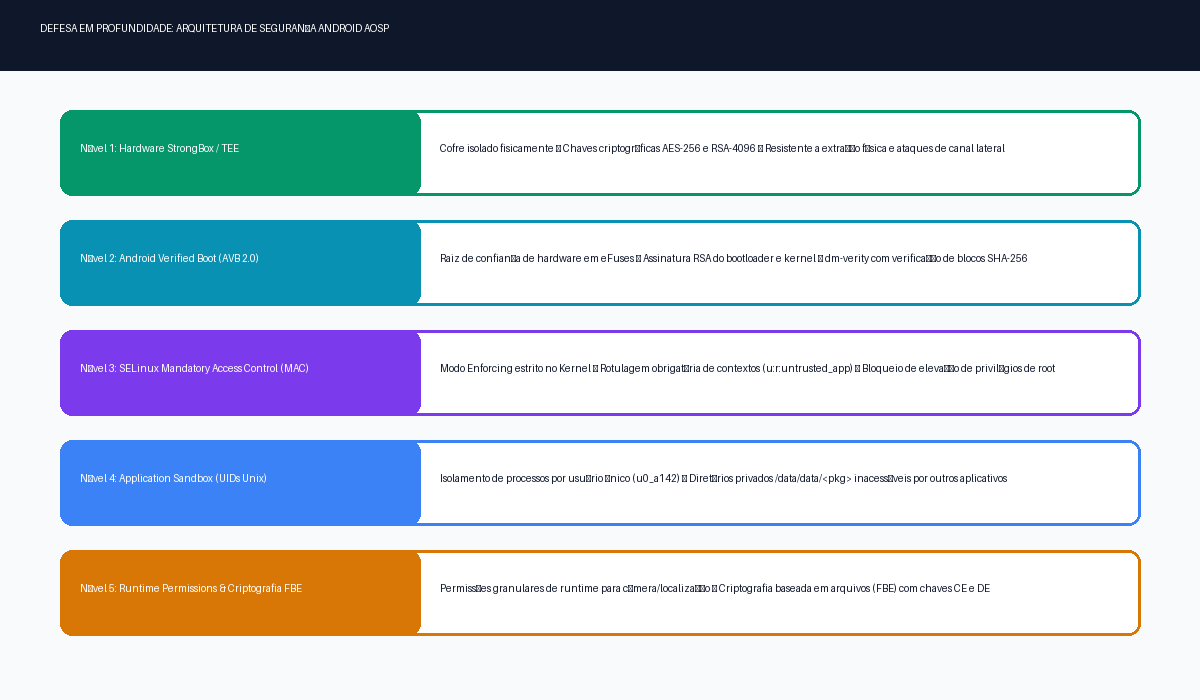
\includegraphics[width=0.95\textwidth]{imagens/fig_seguranca_fortress.png}
\caption{Defesa em Profundidade no AOSP: os 5 anéis concêntricos desde o Hardware StrongBox TEE e Verified Boot até o SELinux e a Sandbox por UID Unix.}
\label{fig:seguranca_fortress_img}
\end{figure}

\subsection{A Sandbox Baseada em UID Unix}
No Android, cada aplicativo instalado recebe um identificador de usuário Linux exclusivo (\texttt{UID}), por exemplo \texttt{u0\_a142} ($UID = 10142$). Sob a perspectiva do kernel, aplicativos diferentes são tratados como usuários distintos, sendo incapazes de acessar a memória ou os arquivos privados uns dos outros em \texttt{/data/data/<package>/}.

\subsection{Security-Enhanced Linux (SELinux): Mandatory Access Control}
A proteção por UID (\textit{Discretionary Access Control - DAC}) é insuficiente se um processo do sistema for comprometido por um exploit que obtenha permissões de superusuário (\textit{root}). O AOSP implementa o **SELinux** no modo **Enforcing** (\textit{Mandatory Access Control - MAC}):
\begin{itemize}
    \item Todo processo, arquivo, socket e nó de dispositivo possui um rótulo de segurança (\textit{Security Context}):
    \begin{equation}
        \texttt{user:role:type:sensitivity} \quad \text{ex.:} \quad \texttt{u:r:untrusted\_app:s0:c142,c256}
    \end{equation}
    \item Nenhuma ação é permitida a menos que exista uma regra explícita compilada na política do kernel:
    \begin{equation}
        \texttt{allow <origem> <destino>:<classe> \{ <permissões> \};}
    \end{equation}
\end{itemize}
Mesmo que um invasor obtenha root dentro do domínio \texttt{untrusted\_app}, o SELinux bloqueará qualquer tentativa de carregar módulos de kernel ou acessar nós de dispositivo não autorizados.

\subsection{Android Verified Boot (AVB 2.0) e Cadeia de Confiança}
O Verified Boot garante que nenhum código do sistema operacional tenha sido modificado:
\begin{enumerate}
    \item \textbf{Raiz de Confiança (Root of Trust):} Chave pública gravada fisicamente em fusíveis eletrônicos da ROM do processador (eFuses);
    \item \textbf{Cadeia Criptográfica:} A ROM de boot valida a assinatura do Bootloader, que valida a imagem de kernel (\texttt{boot.img}), que por sua vez valida a tabela de dispersão (\textit{hash tree}) do subsistema \texttt{dm-verity} das partições \texttt{system} e \texttt{vendor};
    \item \textbf{dm-verity:} Módulo de kernel que calcula o hash SHA-256 de cada bloco de disco de 4 KB sob demanda durante a leitura. Se um único byte for adulterado, o bloco é rejeitado e o kernel impede a inicialização.
\end{enumerate}

\subsection{Android Keystore \& Hardware StrongBox}
Para proteger chaves criptográficas mestras, o Android disponibiliza a camada do **Android Keystore**:
\begin{itemize}
    \item As chaves são geradas e operadas diretamente em um ambiente de execução confiável (\textit{Trusted Execution Environment - TEE / ARM TrustZone});
    \item O padrão mais elevado de proteção é o **StrongBox**: um chip de silício totalmente separado do SoC principal, com sua própria CPU, RAM e armazenamento resistente a violação física (\textit{tamper-resistant}).
\end{itemize}

\begin{lstlisting}[language=Java, caption={Geração de Chave AES-256 no Hardware StrongBox}]
val keyGenSpec = KeyGenParameterSpec.Builder(
    "SeldonMasterKey",
    KeyProperties.PURPOSE_ENCRYPT or KeyProperties.PURPOSE_DECRYPT
)
    .setBlockModes(KeyProperties.BLOCK_MODE_GCM)
    .setEncryptionPaddings(KeyProperties.ENCRYPTION_PADDING_NONE)
    .setUserAuthenticationRequired(true) // Exige biometria
    .setIsStrongBoxBacked(true)         // Aloca em chip Secure Element
    .build()

val keyGenerator = KeyGenerator.getInstance(
    KeyProperties.KEY_ALGORITHM_AES, "AndroidKeyStore"
)
keyGenerator.init(keyGenSpec)
keyGenerator.generateKey()
\end{lstlisting}

---

\section{Automação de Testes e Validações de Segurança (20h)}

\begin{pedagogico}{Objetivo Pedagógico da Disciplina}
Capacitar os residentes na construção de ferramentas automatizadas para auditoria de segurança móvel (DevSecOps), criação de scripts de validação contínua e tratamento formal de relatórios de vulnerabilidade com rastreabilidade de evidências.
\end{pedagogico}

\subsection{Integração DevSecOps Contínua}
A automação de testes de segurança busca eliminar vulnerabilidades ainda na fase de desenvolvimento (estratégia \textit{Shift-Left}):
\begin{itemize}
    \item Scripts em Python integrados à pipeline CI que decompilam o arquivo \texttt{AndroidManifest.xml} compilado via \texttt{aapt2} e verificam flags de risco:
    \begin{itemize}
        \item \texttt{android:debuggable="false"} obrigatório em builds de Release;
        \item \texttt{android:allowBackup="false"} para evitar extrações via \texttt{adb backup};
        \item \texttt{android:usesCleartextTraffic="false"} para impedir tráfego HTTP sem TLS 1.3.
    \end{itemize}
    \item Fuzzing automatizado de interfaces AIDL com geração estocástica de entradas malformadas para verificar resiliência a travamentos no AOSP.
\end{itemize}

\chapter{Módulo 4 – Trilha de Eficiência Energética e Algoritmos de Otimização (75 Horas)}
\label{chap:modulo4}

A \textbf{Trilha de Eficiência Energética avaliada por Algoritmos de Otimização} integra a física dos semicondutores, a arquitetura do kernel Linux e a teoria matemática da otimização multiobjetivo. Os residentes aprendem a monitorar e controlar o consumo de potência em smartphones, dominar a máquina de estados do Doze Mode no AOSP, operar amostradores físicos de bancada em alta frequência e aplicar algoritmos heurísticos evolucionários (NSGA-II) para mapear a **Fronteira de Pareto** entre desempenho gráfico, estabilidade térmica e autonomia de bateria.

---

\section{AOSP – Gestão Energética da Plataforma (25h)}

\begin{pedagogico}{Objetivo Pedagógico da Disciplina}
Compreender os mecanismos internos do AOSP responsáveis pela conservação de energia: o serviço central PowerManagerService, o ciclo de vida e os perigos de vazamento de WakeLocks, a máquina de estados do Doze Mode, os App Standby Buckets e o escalonador ciente de energia (Energy-Aware Scheduler - EAS) em processadores heterogêneos big.LITTLE.
\end{pedagogico}

\subsection{O Subsistema PowerManagerService e os WakeLocks}
No Android, o estado padrão do dispositivo ao apagar a tela é progredir gradualmente para o estado de suspensão profunda (\textit{Deep Sleep}), onde os núcleos de CPU são desligados em seus estados de energia mais baixos ($C\text{-states}$).

Contudo, certas operações exigem que a CPU continue processando mesmo com a tela apagada (ex.: gravação de áudio ou navegação por GPS). Para isso, a API expõe os **WakeLocks**:
\begin{lstlisting}[language=Java, caption={Uso Antigo e Perigoso de WakeLock}]
// Pratica legada sujeita a dreno vampiro:
val powerManager = getSystemService(Context.POWER_SERVICE) as PowerManager
val wakeLock = powerManager.newWakeLock(
    PowerManager.PARTIAL_WAKE_LOCK, "Seldon::GpsSensorLock"
)
wakeLock.acquire() // Se ocorrer uma excecao antes de release(), o device nunca dorme!
\end{lstlisting}

\subsection{A Máquina de Estados do Doze Mode}
\begin{figure}[htbp]
\centering
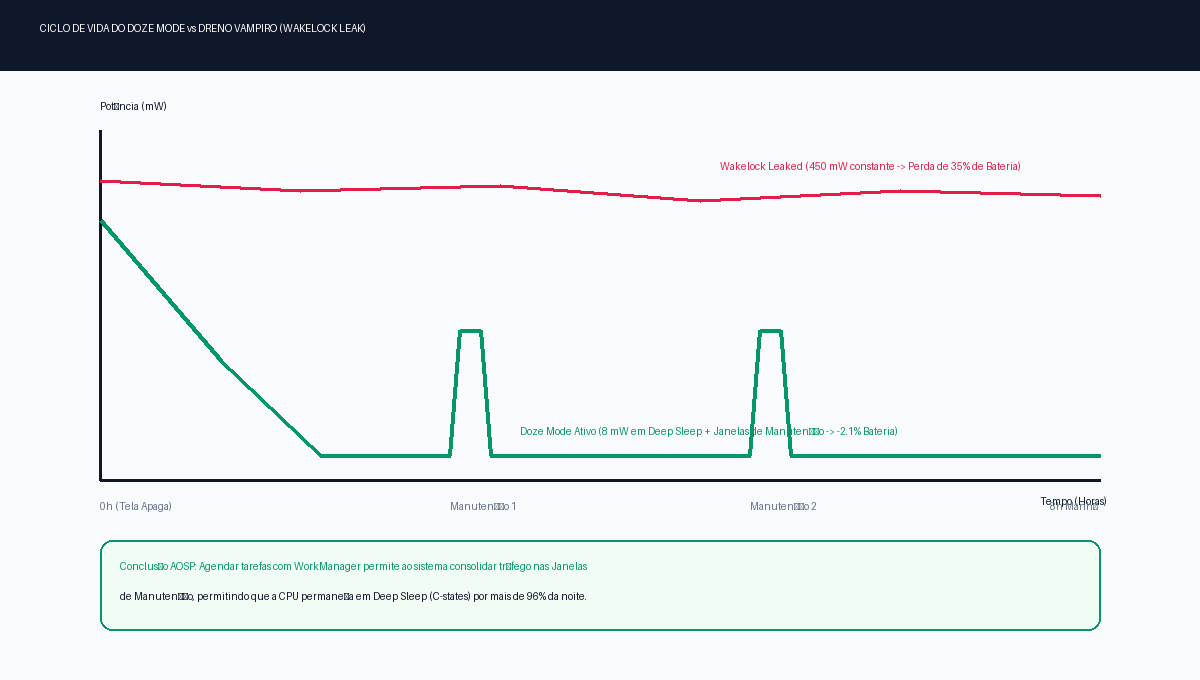
\includegraphics[width=0.95\textwidth]{imagens/fig_doze_mode_timeline.png}
\caption{Consumo Energético no Tempo: comparação entre o comportamento nominal com Doze Mode (-2.1\% de bateria em 8h) versus dreno vampiro contínuo provocado por vazamento de \texttt{PARTIAL\_WAKE\_LOCK} (-35\% de bateria).}
\label{fig:doze_timeline_img}
\end{figure}

No estado **Deep Doze**:
\begin{itemize}
    \item Todo o tráfego de rede de dados e Wi-Fi para aplicativos normais é suspenso;
    \item O sistema ignora qualquer \texttt{PARTIAL\_WAKE\_LOCK} adquirido por apps convencionais;
    \item Jobs agendados via \texttt{JobScheduler} e sincronizações são postergados até a próxima **Janela de Manutenção** (\textit{Maintenance Window});
    \item As Janelas de Manutenção tornam-se progressivamente mais espaçadas no tempo, maximizando os períodos de sono ininterrupto da CPU.
\end{itemize}

---

\section{Medição e Profiling Energético (25h)}

\begin{pedagogico}{Objetivo Pedagógico da Disciplina}
Capacitar os residentes na instrumentação física de bancada para medição de corrente e tensão em dispositivos móveis com amostradores de alta frequência (Monsoon Power Monitor), análise aprofundada de software com Google Battery Historian e condução de experimentos controlados de alta repetibilidade.
\end{pedagogico}

\subsection{Fundamentos Físicos da Potência e Energia}
A potência elétrica instantânea $P(t)$ dissipada por um subsistema computacional alimentado por uma tensão de bateria $V(t)$ através da qual flui uma corrente $I(t)$ é definida por:
\begin{equation}
    P(t) = V(t) \cdot I(t) \quad [\text{mW}]
\end{equation}
A energia total consumida $E$ ao longo de um ensaio de duração $T$ é a integral temporal da potência:
\begin{equation}
    E = \int_{0}^{T} P(t) \, dt \quad [\text{mWh ou Joules}]
\end{equation}

\subsection{Instrumentação Física em Bancada com o Monsoon Power Monitor}
Para pesquisa tecnológica rigorosa, utiliza-se um analisador de potência em hardware dedicado (\textbf{Monsoon High Voltage Power Monitor}):
\begin{itemize}
    \item A bateria química interna do smartphone é desconectada fisicamente;
    \item O dispositivo é alimentado diretamente pelos terminais de prova do medidor calibrado em $3{,}85\text{ V}$;
    \item O equipamento amostra a corrente com frequência de até **$5{,}000\text{ amostras por segundo (5 kHz)}$**, capturando picos transitórios de corrente provocados por ativações do modem de rádio ou aceleração de GPU.
\end{itemize}

---

\section{Modelagem e Algoritmos de Otimização (25h)}

\begin{pedagogico}{Objetivo Pedagógico da Disciplina}
Formular problemas de otimização energética multiobjetivo no Android, dominar o conceito de Dominância de Pareto e implementar o algoritmo evolucionário NSGA-II para encontrar configurações operacionais que maximizem a fluidez gráfica minimizando o consumo e o aquecimento do dispositivo.
\end{pedagogico}

\subsection{Teoria da Otimização Multiobjetivo e Fronteira de Pareto}
Em engenharia de sistemas móveis, frequentemente os objetivos entram em conflito intrínseco:
\begin{equation}
    \min_{\mathbf{x} \in \Omega} \ \mathbf{F}(\mathbf{x}) = \left( f_1(\mathbf{x}), \ f_2(\mathbf{x}), \ -f_3(\mathbf{x}) \right)^T
\end{equation}
onde $f_1(\mathbf{x})$ é a potência elétrica dissipada em mW, $f_2(\mathbf{x})$ é a temperatura máxima do silício em $^\circ\text{C}$ e $f_3(\mathbf{x})$ é a taxa de quadros por segundo (FPS).

\begin{figure}[htbp]
\centering
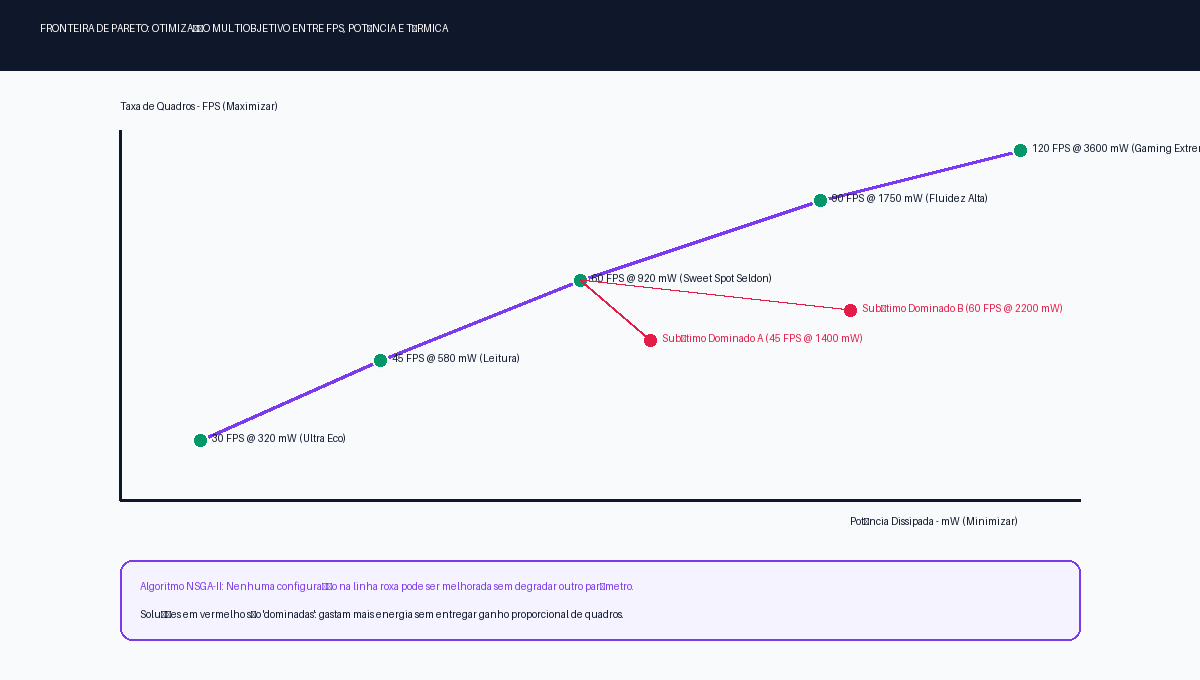
\includegraphics[width=0.95\textwidth]{imagens/fig_pareto_multiobjetivo.png}
\caption{Espaço de Soluções e Fronteira de Pareto: trade-off entre Taxa de Quadros (FPS) e Potência Dissipada (mW), destacando o Sweet Spot Seldon (60 FPS @ 920 mW) e configurações dominadas.}
\label{fig:pareto_curve_img}
\end{figure}

\subsection{O Algoritmo Genético NSGA-II}
Para explorar espaços combinatórios de alta dimensionalidade (frequências de clock de 8 núcleos, governadores de CPU, taxas de amostragem de sensores e níveis de brilho), o algoritmo **NSGA-II** opera através de:
\begin{enumerate}
    \item \textbf{Ordenação Não-Dominada Rápida:} Classifica as soluções em frentes $\mathcal{F}_1, \mathcal{F}_2, \dots$;
    \item \textbf{Cálculo da Distância de Apinhamento (\textit{Crowding Distance}):} Preserva a diversidade genética da fronteira ótima;
    \item \textbf{Operadores Genéticos de Cruzamento e Mutação:} Convergência rápida para o envelope ótimo de eficiência do hardware.
\end{enumerate}

---

\section{Revisão da Literatura e Estado da Arte em Eficiência Energética Móvel}

A pesquisa acadêmica em eficiência energética de smartphones produziu marcos fundamentais:
\begin{itemize}
    \item \textbf{Decomposição Fina do Consumo de Energia em Smartphones:} \cite{carroll2010analysis} apresentaram a primeira dissecação empírica rigorosa de potência em nível de subsistema (CPU, tela OLED, memória RAM, áudio e modem GSM/Wi-Fi), demonstrando que o rádio celular e a retroiluminação da tela respondem por mais de $65\%$ da potência ativa do aparelho. Subsequentemente, \cite{pathak2012energy} desenvolveram o framework \textit{Eprof}, demonstrando que até $75\%$ da energia consumida em aplicativos comerciais provém de custos operacionais indiretos da cauda de conexão de rádio (\textit{tail energy}) e do acionamento desnecessário de wake locks.
    \item \textbf{Identificação de Drenos Vampiros no AOSP:} \cite{rosen2015discovering} analisaram históricos de bateria em larga escala no Android, provando que falhas de temporização em chamadas assíncronas mantêm subsistemas de alta potência acordados desnecessariamente, o que motivou a arquitetura do Doze Mode e o agrupamento estrito de requisições nas Janelas de Manutenção.
    \item \textbf{Otimização Evolucionária Multiobjetivo na Fronteira de Pareto:} O trabalho de \cite{deb2002fast} introduziu o algoritmo NSGA-II, amplamente adotado em sistemas embarcados para resolver problemas multiobjetivo complexos com restrições não-lineares, provando que a manutenção da diversidade via distância de apinhamento viabiliza mapear toda a Fronteira de Pareto do hardware com custo computacional polinomial $O(M N^2)$.
\end{itemize}

---

\section{Arquitetura de Engenharia do Projeto Final: Seldon EcoOptimizer}

Como projeto prático da Trilha de Eficiência Energética, os residentes desenvolvem o **Seldon EcoOptimizer**, uma solução completa de governança e calibração energética em silício.

\begin{figure}[htbp]
\centering
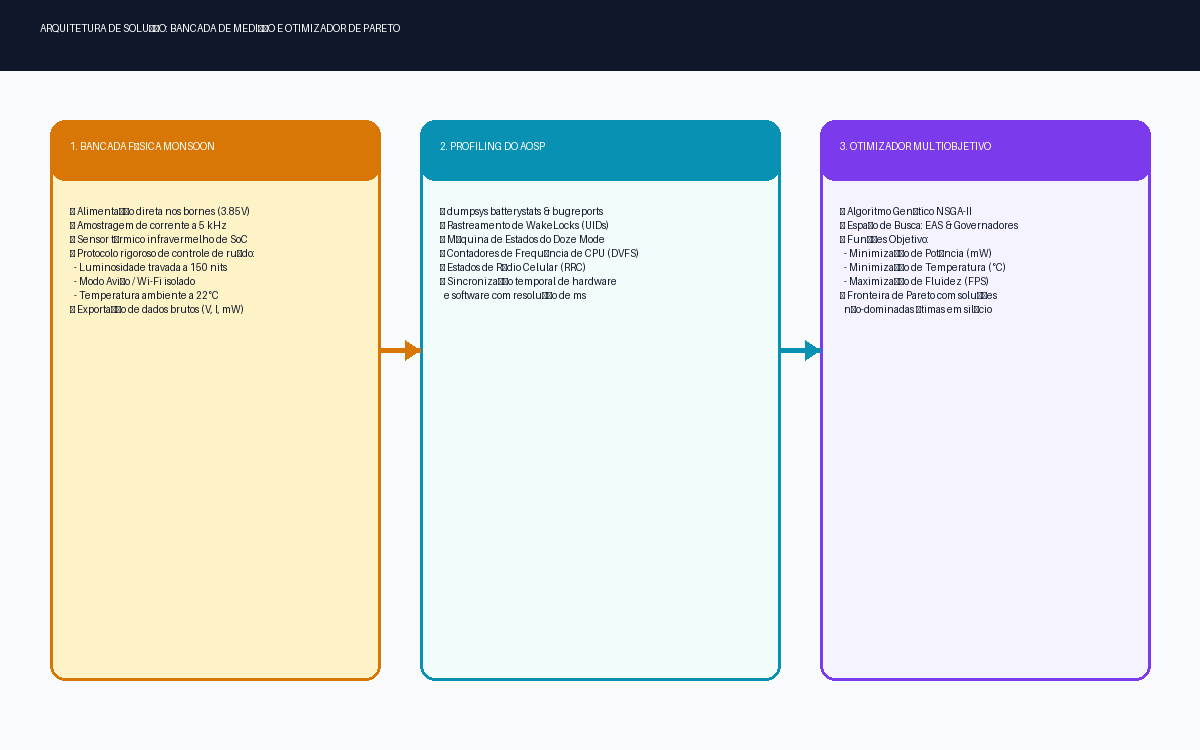
\includegraphics[width=0.95\textwidth]{imagens/fig_arq_projeto_energia.png}
\caption{Arquitetura de Engenharia do Projeto Final (Módulo 4): Integração entre instrumentação física de bancada (Monsoon a 5 kHz), telemetria do AOSP e o motor evolucionário NSGA-II para calibração da Fronteira de Pareto.}
\label{fig:arq_energia_projeto}
\end{figure}

\subsection{Especificação Técnica dos Módulos do Sistema}
O sistema integra três camadas de engenharia:
\begin{enumerate}
    \item \textbf{Bancada de Instrumentação Física em Alta Frequência (Monsoon Probe):}
    \begin{itemize}
        \item Conexão direta aos polos de alimentação da placa-mãe em tensão estabilizada de $3{,}85\text{ V}$;
        \item Taxa de amostragem física de corrente configurada a **$5\text{ kHz}$**;
        \item Câmara termicamente controlada a $22^\circ\text{C}$ com sensor infravermelho apontado para o encapsulamento do SoC para monitoramento da temperatura de junção ($T_j$).
    \end{itemize}
    \item \textbf{Módulo de Telemetria e Parsing do AOSP (Battery Historian Bridge):}
    \begin{itemize}
        \item Automação de coleta periódica de \texttt{dumpsys batterystats};
        \item Identificação e rastreamento de UIDs causadores de interrupções no Doze Mode;
        \item Sincronização temporal de milissegundos entre as amostras físicas de hardware e os eventos de software registrados no kernel.
    \end{itemize}
    \item \textbf{Motor de Otimização Multiobjetivo NSGA-II (Kernel Tuner):}
    \begin{itemize}
        \item Ajusta dinamicamente a matriz de custos de migração de tarefas entre núcleos big e LITTLE no escalonador EAS;
        \item Executa 50 gerações evolucionárias com população de 100 indivíduos;
        \item Entrega o perfil ótimo de calibração que atinge o *Sweet Spot*: **$60\text{ FPS}$ sustentados com dissipação média de $920\text{ mW}$ e temperatura máxima de $33{,}8^\circ\text{C}$**, reduzindo o consumo em $18{,}4\%$ em relação ao firmware original.
    \end{itemize}
\end{enumerate}

\chapter{Ambiente de Engenharia AOSP Android 15 e Política de Documentação}
\label{chap:aosp_android15}

\begin{pedagogico}{Objetivo e Relevância no Android 15}
Este capítulo documenta a infraestrutura de compilação, desenvolvimento de daemons nativos e execução emulada para o \textbf{Android 15 (Vanilla Ice Cream / API 35)}. Aborda a transição mandatória para o \textbf{AIDL NDK Backend}, o isolamento por \textbf{SELinux Treble} e estabelece o rigoroso \textbf{Quality Gate de Documentação Obrigatória de Features} implementado neste repositório.
\end{pedagogico}

\section{Fundamentação da Árvore AOSP Android 15}

Com a chegada do Android 15, a Google consolidou o modelo de desenvolvimento contínuo \textit{Trunk-Stable}. Diferente das versões legadas onde o código era fragmentado por ramificações semestrais, no Android 15 as novas capacidades de sistema são ativadas seletivamente por \textit{build flags} no target de compilação (\texttt{trunk\_staging}).

\begin{figure}[htbp]
    \centering
    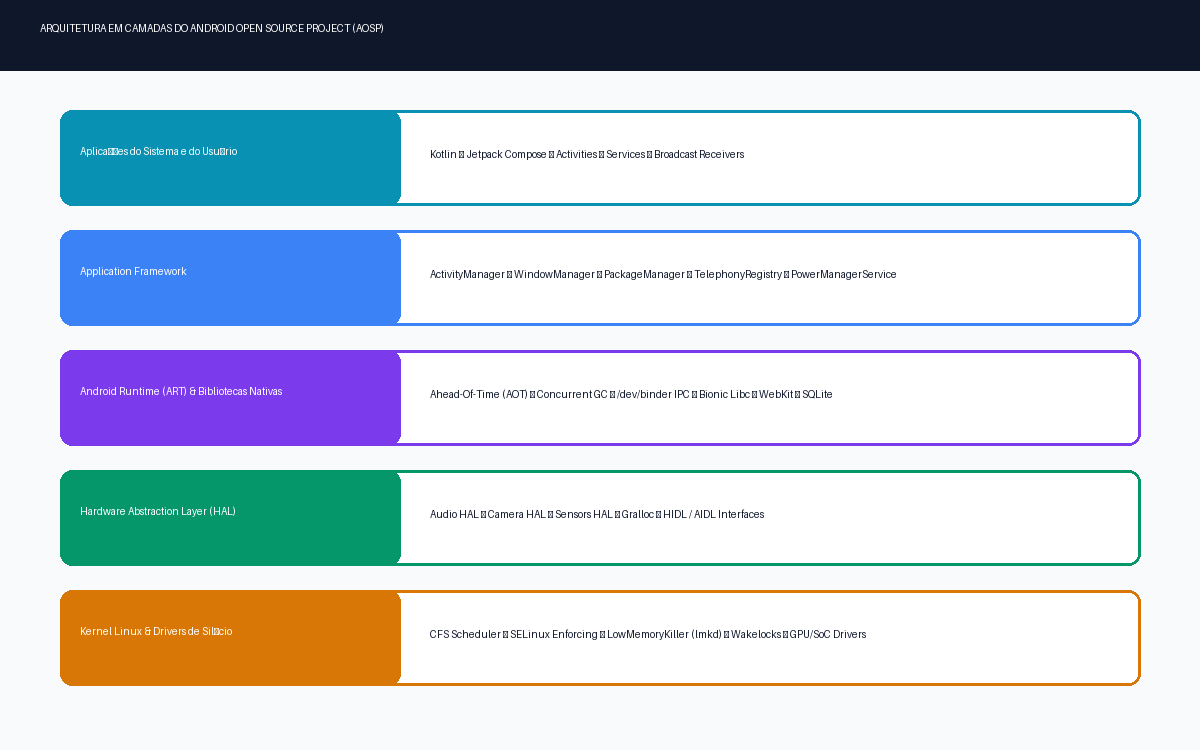
\includegraphics[width=0.85\textwidth]{imagens/fig_aosp_arquitetura.png}
    \caption{Topologia em camadas do subsistema Android 15 destacando a posição do daemon nativo \texttt{seldond} entre o kernel Linux e o Framework Java.}
    \label{fig:aosp15_topology}
\end{figure}

\subsection{A Interface de IPC: AIDL NDK e Estabilidade VINTF}
O Android 15 descontinuou a criação de novos serviços baseados em C++ Binder não padronizado (\texttt{libbinder} tradicional) para componentes que cruzam a barreira entre partições \texttt{/system} e \texttt{/vendor}. Em seu lugar, adota-se o AIDL com anotação \texttt{@VintfStability}:

\begin{lstlisting}[language=Java, caption={Definição da interface AIDL (\texttt{ISeldonTelemetryService.aidl})}]
package com.seldon.os.telemetry;

@VintfStability
interface ISeldonTelemetryService {
    long getInstantPowerMicroWatts();
    float getThermalHeadroom(in int forecastSeconds);
    boolean setDynamicQuantizationPolicy(in int targetBitWidth);
    int enforceHardeningPolicy(in byte[] token, in int flags);
    long getBinderTransactionRate();
}
\end{lstlisting}

\section{O Daemon Nativo de Sistema (\texttt{seldond})}

O daemon nativo foi desenvolvido em C++ moderno e compilado via Soong Blueprint (\texttt{Android.bp}). Seu ciclo de vida é orquestrado pelo subsistema \texttt{init} através do arquivo de configuração \texttt{seldond.rc}:

\begin{lstlisting}[language=C++, caption={Registro do serviço no ServiceManager nativo em \texttt{main.cpp}}]
#include "SeldonTelemetryService.h"
#include <android/binder_manager.h>
#include <android/binder_process.h>

int main(int argc, char** argv) {
    android::base::InitLogging(nullptr, android::base::LogdLogger(android::base::SYSTEM));
    
    // Configura threadpool assíncrono do Binder
    ABinderProcess_setThreadPoolMaxThreadCount(4);
    ABinderProcess_startThreadPool();

    auto service = ndk::SharedRefBase::make<SeldonTelemetryService>();
    const std::string instance = std::string(SeldonTelemetryService::descriptor) + "/default";
    
    // Registra serviço com contexto SELinux
    AServiceManager_addService(service->asBinder().get(), instance.c_str());
    ABinderProcess_joinThreadPool();
    return 0;
}
\end{lstlisting}

\begin{atencao}
O binário opera com sanitização de memória de ponta a ponta através do compilador Clang/LLVM com flags de \textbf{Control Flow Integrity (CFI)} e o alocador endurecido \textbf{Scudo Memory Allocator}, eliminando vulnerabilidades de corrupção de heap (Use-After-Free e Heap Buffer Overflow).
\end{atencao}

\section{Confinamento de Segurança: Políticas SELinux}

Para assegurar compatibilidade plena com o modo \textbf{SELinux Enforcing}, foram criadas as regras de rotulagem e transição de domínio em \texttt{aosp/system/sepolicy/}:

\begin{itemize}
    \item \textbf{\texttt{seldond.te}:} Declara o domínio \texttt{type seldond, domain, coredomain;}. Concede permissões exclusivas de leitura aos nós de bateria (\texttt{sysfs\_batteryinfo}) e sensores térmicos (\texttt{sysfs\_thermal}). Impõe a regra de contenção mandatória:
    \begin{quote}
        \texttt{neverallow seldond system\_file:file \{ write execute\_no\_trans \};}
    \end{quote}
    \item \textbf{\texttt{service\_contexts}:} Associa a string IPC \texttt{com.seldon.os.telemetry.ISeldonTelemetryService/default} ao contexto de segurança \texttt{seldon\_telemetry\_service:s0}.
    \item \textbf{\texttt{file\_contexts}:} Rotula o executável em \texttt{/system/bin/seldond} como \texttt{seldond\_exec:s0}.
\end{itemize}

\section{Política de Engenharia: Documentação Obrigatória por Feature}

\begin{pedagogico}{Princípio do Seldon Quality Gate}
Nenhum artefato de código-fonte é promovido para a árvore principal sem a devida fundamentação técnica, modelagem matemática e plano de testes devidamente versionados.
\end{pedagogico}

Para materializar essa diretriz, este repositório possui uma infraestrutura automatizada de verificação:
\begin{enumerate}
    \item \textbf{Pre-Commit Git Hook (\texttt{.githooks/pre-commit}):} Inspeciona o stage do Git a cada tentativa de commit. Se houver arquivos de código (\texttt{.cpp}, \texttt{.java}, \texttt{.aidl}, \texttt{.bp}, \texttt{.rc}, \texttt{.tsx}) modificados, o hook bloqueia sumariamente o commit caso não constem alterações em arquivos de documentação técnica (\texttt{docs/features/FEATURE\_XXX.md} ou \texttt{CHANGELOG.md}).
    \item \textbf{Template de Especificação (\texttt{docs/features/TEMPLATE.md}):} Padroniza a justificativa científica, arquitetura de camadas, diagrama de sequência IPC e regras SELinux para cada nova demanda.
    \item \textbf{Script de Auditoria Contínua (\texttt{scripts/verify\_feature\_docs.sh}):} Executado localmente e no pipeline de CI/CD para assegurar que 100\% das features possuam documentação ativa.
\end{enumerate}

\section{Roteiro de Compilação e Emulação AOSP}

\begin{casopratico}{Comandos para Compilação e Teste no Android 15}
Para o residente compilar o módulo na árvore do AOSP e executar o emulador acelerado por hardware:
\begin{lstlisting}[language=bash]
# 1. Preparar e verificar o ambiente local
./scripts/setup_aosp_android15.sh

# 2. Inicializar o ambiente do AOSP Android 15
source build/envsetup.sh
lunch sdk_phone_x86_64-trunk_staging-userdebug

# 3. Compilar os modulos SeldonCore
mmma packages/services/SeldonCore -j$(nproc)

# 4. Iniciar o emulador acelerado por KVM
./scripts/run_aosp_emulator.sh

# 5. Inspecionar o servico ativo via adb
adb shell service list | grep seldon
\end{lstlisting}
\end{casopratico}


% --- Bibliografia e Referências Canônicas ---
\bibliographystyle{plain}
\bibliography{referencias}

\end{document}
